\chapter{Lexical Entailment Detection with H-features}
\label{ch:hpm}

This chapter shows new model of lexical relationship predictions, and related
material. The work in this chapter has been published in
\newcite{roller:2016:emnlp}.

\section{Chapter Overview}

In the previous chapter, we considered one novel model for hypernymy detection,
and showed how experimental setup can vastly affect one's conclusions about
effectiveness of models on this task. Since then, most work has considered the
importance of experimental setup and lexical overlap, and a plethora of
supervised distributional approaches have been proposed for different variations
of the task.

In this chapter, we review additional work on supervised relationship
prediction using distributional semantics, and consider the strengths of
different models in the literature. We consider how the construction of
distributional spaces affects model performance, especially within the
framework of prototypicality analysis discussed in the previous chapter. We
find that hypernymy detection classifiers have a high degree of
interpretability when considered carefully.  We propose a novel model which
combines the advantages of prototypicality classifiers, while addressing their
pitfalls. Our new model achieves consistently strong or state-of-the-art
performance across numerous datasets, including datasets of hypernymy
detection, general lexical entailment, and multi-relation classification.

\section{Related Work for Supervised Models}

\begin{comment}
  classification:
    -- baroni:2012:eacl
    -- roller:2014:coling
    -- weeds:2014:coling
    -- levy:2015:naacl
    -- kruszewski:2015:tacl
    -- shwartz:2016:acl
    turney:2015:nle
  multi relation:
    vylomova:2016:acl
    swhartz:2016:cogalex1
    shwartz:2016:cogalex2
  multi language
    bordea:2016:semeval
  regression:
    espinosaanke:2016:emnlp
    nayak:2015:techreport
    fu:2014:acl
\end{comment}

In the previous chapter, we considered many models for lexical entailment and
hypernymy detection, especially those based on the frameworks of Hearst
patterns and unsupervised distributional measures based on the Distributional
Inclusion Hypothesis. Here we focus only on the {\em supervised} approaches of
lexical entailment using distributional semantics, and attempt to highlight
the differences and considerations of the many approaches.

As discussed earlier, the earliest supervised approach was that of
\newcite{baroni:2012:eacl}, who used an off-the-shelf polynomial SVM train on
the {\em concatenation} of the pair $\wordpair$. Such a model obtains strong
performance on randomized stratifications of datasets, but performs poorly
when testing for lexical generalization. This issue was observed simultaneously
by \newcite{roller:2014:coling} and \newcite{weeds:2014:coling}, who published
these concerns at the same conference. The former approached the problem
through the stratification methods described earlier, but the latter considered
how well models perform over a random vector experiment. That is, models were
trained both on real distributional vectors and {\em randomized} distributional
vectors. Models which had little difference between their real and randomized
results were assumed to be memorizing the data, while models which improved
upon the random vectors were considered strong. This is a very different
approach to issues of lexical memorization. We consider this experimental
setup to be inadequate, since randomized vectors are unable to exploit the
distributional hypothesis, and therefore systematically underestimate the
robustness of some models. Nonetheless, they report strong results for linear
models using either vector concatenation (Concat) or vector difference (Diff)
input representations, but consider the Concat representation superior.

\newcite{levy:2015:naacl} focus particularly on the issue of lexical
memorization, and seek to elaborate on what kinds of models are subject to
these issues. They emphasize the importance of the inner product terms in
generalizing to novel words, and propose the notion of {\em prototypicality},
suggesting that some models merely look to identify words which appear like the
most prototypical hypernym or hyponym, regardless actual relation. They
therefore conclude that specific linear models (like Diff and Concat, but not
Asym) are doomed to this behavior through the analysis we saw in the previous
chapter. They also propose {\em Ksim}, a specialized nonlinear SVM kernel which
explicitly includes the critical similarity term which Concat and Diff lack.
Their views on prototypicality will inform and motivate our model proposed in
this chapter.

\newcite{kruszewski:2015:tacl} focus more strongly on the role of the
Distributional Inclusion Hypothesis within the framework of supervised models,
and propose a custom neural network for lexical entailment. In particular, they
focus on projecting the distributional space into latent boolean features where
the Distributional Inclusion Hypothesis maximally holds. They compare their
model with a carefully tuned SVM with an RBF kernel, and find mixed results
regarding which is stronger. However, they find the latent subspace induced
by their model contains highly interpretable word clusters, and provide additional
evidence for the Distributional Inclusion Hypothesis.

\newcite{shwartz:2016:acl} consider whether traditional path-based
approaches may be improved using the lessons learned from distributional
approaches. They propose a Recurrent Neural Network approach which trains
an LSTM \cite{hochreiter:1997:nc} on dependency paths between $h$ and $w$.
These recurrent paths are pooled and concatenated with distributional
representations, showing an improvement over comparable path-only and
distributional-only baselines.

Some other works have considered whether it is possible to learn a {\em
regression} from hyponyms to hypernyms. In particular, \newcite{fu:2014:acl}
attempt the regression using vector differences, but find that separate
regression models must be trained for separate regions of distributional
space found via $k$-means clustering. \newcite{espinosaanke:2016:emnlp} find
the clustering step better corresponds to domain-specificity, and propose
learning separate regressions per-domain rather than per-cluster, showing
substantial improvement.  \newcite{nayak:2015:techreport} attempts to
circumvent the domain specificity issue entirely using deep feed-forward neural
networks, and find moderate improvements in precision over a baseline linear
model.

Other works consider whether results from hypernymy detection generalize to
other types of lexical relationships, including other taxonomic relations
like meronomy or co-hyponymy, but also other interesting semantic relations
like cause-effect, agent-object or time-activity. \newcite{vylomova:2016:acl}
finds that a linear model trained on vector differences is able to successfully
distinguish between many lexical relations, including hypernymy, meronomy,
gender (\lit{king/queen}), object-location (\lit{fish/aquarium}), and
action-object (\lit{zip/coat}). They also find that additional negative
sampling (via pair randomization) can improve performance, and that difference
vectors are robust across several models of distributional spaces.
Additionally, Shwartz and Dagan~(\shortcite{shwartz:2016:cogalex2,shwartz:2016:cogalex1})
apply the hybrid path-and-distributional neural
net \cite{shwartz:2016:acl} to multi-relation datasets and again find that
hybrid approaches generally outperform only-path or only-distributional
approaches, though the differences are less pronounced than in hypernymy-only
datasets.

\section{Understanding Distributional Hypernymy Detectors}

In the reviewed literature above, we saw that many models have been considered
across a large variety of experiments and setups. However, different works have
come to different conclusions about the strengths and weaknesses of specific
models. Namely, the Diff and Concat models have had a smattering of seemingly
contradictory results: some papers find that vector differences better capture
lexical relationships \cite{fu:2014:acl,roller:2014:coling,vylomova:2016:acl},
while others suggest that simple concatenation is better
\cite{baroni:2012:eacl,weeds:2014:coling,shwartz:2016:acl}. To make matters
more confusing, the analysis of \newcite{levy:2015:naacl} suggest that
{\em neither} should be able to perform well, as both measure prototypicality
and fail to model relationships directly; yet empirically, both models do
significantly better than chance, and successfully generalize in adversarial
experiments with zero lexical overlap.

We aim to understand why these linear, prototypicality models are able to
perform the task at all. To this end, we now study Concat extensively, and
propose an alternative view of prototypicality: rather than simply modeling the
``average'' hypernym or hyponym, Concat actually acts as a kind of feature
extractor which detects {\em aspects} typical of hypernyms.  We study these
properties by focusing only on binary classification experiments.

We focus on four different datasets, two of which are hypernymy-only datasets, and the remaining two are general lexical entailment datasets. The first
two datasets are {\bf LEDS} and {\bf BLESS}, which contain both positive and
negative examples of hypernymy, as discussed in the previous chapter. However,
here we explicitly binarize the BLESS dataset such that all hypernymy examples
in BLESS are labeled as positive, while random and other relations are labeled
as negative. LEDS only contains hypernymy and non-hypernymy examples, and so is
already binary.

The next dataset we consider is {\bf Medical} \cite{levy:2014:conll}. This
dataset contains noisy annotations of subject-verb-object entailments
extracted from medical texts, and transformed into noun-noun entailments by
argument alignments. The data contains 12,600 annotations, but only 945
positive examples encompassing various relations like hypernymy, meronomy,
synonymy, and some examples of ``contextonymy,'' or entailments that occur in
{\em some} specific contexts, but do not cleanly fit in other categories (e.g.
\lit{hospital} entails \lit{doctor}). It one of the most difficult datasets:
it is both highly domain specific (containing mostly medical terms) and highly
unbalanced.

The final dataset we consider is {\bf TM14}, a variation on the SemEval 2012
Shared Task of identifying the degree to which word pairs exhibit various
relations. These relationships include a small amount of hypernymy, but also
many more uncommon relations (agent-object, cause-effect, time-activity, etc).
Relationships were binarized into (non-)entailing pairs by
\newcite{turney:2015:nle}.  The dataset covers 2188 pairs, 1084 of which are
entailing.

These two entailment datasets contain important differences, especially in
contrast to the hypernymy datasets. Neither contains any randomly generated
negative pairs, meaning general semantic similarity measures should be less
useful; And both exhibit a variety of non-hypernymy relations, which are less
strictly defined and more difficult to model.

\subsection{Distributional Vectors}

Before we fully analyze Concat, we wish to
describe our choice of distributional space, which will have a profound
repercussions in the next experiment. Namely, we desire to explore whether
syntactic spaces or bag-of-words spaces are better suited for lexical
entailment models. We must consider this directly, as the syntactic space in
the previous chapter was trained on different corpora, and transformed using
Local Mutual Information \cite{evert:2005:phd} rather than PPMI.

We construct several distributional spaces over a corpus containing the
concatenation of Gigaword, Wikipedia, BNC and ukWaC.  We preprocess the corpus
using Stanford CoreNLP 3.5.2 \cite{chen:2014:emnlp} for tokenization,
lemmatization, POS-tagging and universal dependency parses. We compute
distributional vectors for 250k most frequent lemmas (with POS tags) by
counting either their syntactic neighbors in a collapsed dependency parse, or a
fixed bag-of-words window. Syntactic co-occurrences are limited to the one
million most frequent contexts, while bag-of-words were limited to the 20k most
frequent contexts. Co-occurrence counts were transformed using PPMI, and SVD
reduced to 300 dimensions. Finally, all vectors were normalized to unit length.
Altogether, this careful construction makes the vectors more comparable.

With all other factors held constant, we compare the effects chosen context
using a baseline Concat model \cite{weeds:2014:coling} on the four datasets in
an experimental setup comparable to the one in the previous chapter.
Figure~\ref{fig:window} shows the results comparing the choice of window
size across all four datasets. The scores of the syntactic spaces are listed
as a window size of 0.

\begin{figure}
  \centering
  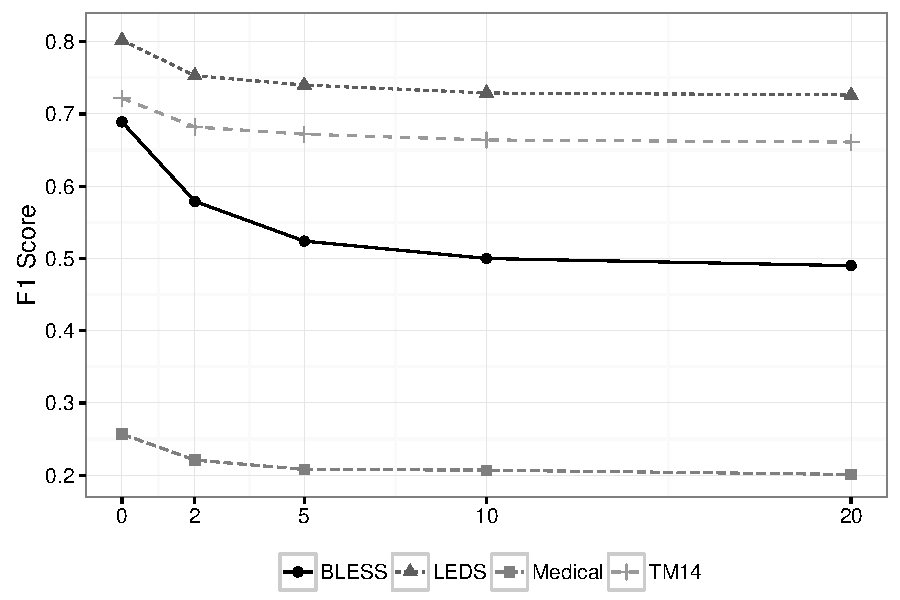
\includegraphics[width=0.75\textwidth]{plots/window.pdf}
  \caption{Comparison of different distributional window sizes for a baseline
  classifier on several different datasets. A window size of 0 contains the
  results for a syntactic distributional space.}
  \label{fig:window}
\end{figure}

Across all four datasets, we see that performance generally degrades as we
increase the size of the context window of our distributional space. Since
syntactic distributional space substantially outperforms the BoW spaces
in all four datasets, we use it in all remaining experiments for this chapter.


%In all experiments, we use a standard, count-based, syntactic distributional
%vector space.  We use a corpus composed of the concatenation of Gigaword,
%Wikipedia, BNC and ukWaC. We compute a syntactic distributional space for
%the 250k most frequent lemmas by counting their dependency neighbors across the
%corpus. We use only the top 1M most frequent dependency attachments as
%contexts.  We use CoreNLP's ``collapsed dependencies'', in which prepositional
%dependencies are collapsed e.g.  ``go to the store'' emits the tuples
%(go,~prep:to+store) and (store,~prep:to\depinv+go).  After collecting counts,
%vectors are transformed using PPMI, SVD reduced to 300 dimensions, and
%normalized to unit length. The use of collapsed, syntactic dependencies for
%co-occurrences is very important, but other parameters are reasonably robust.

\subsection{Reconsidering Prototypicality}

As we saw in the previous chapter, the Concat model, which trains a linear
classifier on the concatenation of word vectors $\pair$ has a fundamental
flaw: that it does not explicitly model any direct interaction term between
$h$ and $w$. Rather, the hyperplane $\vhatp$ may be interpreted as learning
a model of {\em prototypicality}, or how similar $\vh$ is to the prototypical
or average hypernym $\vhath$. We show the analysis here again:
\begin{align}
  \begin{split}
  \vhatp^\top \wordpair & = \protopair^\top \wordpair\\
  & = \vhath^\top\vh + \vhatw^\top\vw\\
  & = \mbox{cos}(\vhath, \vh) + \mbox{cos}(\vhatw, \vw)
  \end{split}
\tag{\ref{eqn:prototypicality} revisited}
\end{align}
As \newcite{levy:2015:naacl} point out, this analysis shows that Concat will
fail on many randomly paired examples, like (\lit{animal},~\lit{cactus}), as
$\litvec{animal}$ is a rather prototypical hypernym, and $\litvec{cactus}$ is
a rather prototypical hyponym (of plant).

We agree with this prototypicality interpretation, although we believe it is incomplete:
while it places a fundamental ceiling on the performance of these classifiers, it
does not explain {\em why} others have found them to persist as strong
baselines
\cite{weeds:2014:coling,roller:2014:coling,kruszewski:2015:tacl,vylomova:2016:acl}.
To approach this question, we consider a baseline Concat classifier trained
using a linear model. This classifier should most strongly exhibit the prototypicality
behavior according to Equation~\ref{eq:proto}, making it the best
choice for analysis. We first consider the most pessimistic hypothesis: is it
only learning to memorize which words are hypernyms at all?

We train the baseline Concat classifier using Logistic Regression on each of
the four datasets, and extract the vocabulary words which are most similar to
the $\hat H$ half of the learned hyperplane $\hat p$. If the classifier is only
learning to memorize the training data, we would expect the most frequent
hypernyms from the data to dominate this list of closest vocabulary terms, as
the centroid $\hat H$ should be strongly located near them.
Table~\ref{tab:wordsim} gives the five most similar words to the learned
hyperplane, with bold words appearing directly in the dataset.

\begin{table}[t]
\begin{center}
  %\begin{small}
  \begin{tabular}{|llll|}
    \hline
    {\bf LEDS} & {\bf BLESS} & {\bf Medical} & {\bf TM14}\\
    \hline
     %% baroni           %% bless             %% levy               %% turney_lemma           \\
     material       &      goods             &     item           &      sensitiveness          \\
     structure      &      lifeform          &     unlockable     &      tactility              \\
     object         & {\bf item}             &     succor         &      palate                 \\
     process        & {\bf equipment}        &     team-up        &      stiffness              \\
     activity       & {\bf herbivore}        &     non-essential  &      content                \\
%     environment    &      omnivore          &     40px           &      ductility              \\
%     element        & {\bf creature}         &     crimefighter   &      musculature            \\
%{\bf practice}      &      life-form         &     material       &      dimensionality         \\
%     nature         & {\bf artifact}         &     assitance      &      quality                \\
%     organism       & {\bf pest}             &     nourishment    &      angulation             \\
    \hline
  \end{tabular}
  %\end{footnotesize}
\end{center}
\caption{Most similar words to the prototype $\vhath$ learned by a Concat model. Bold items
appear in the dataset. Very few of the closest terms directly appear in the dataset.}
\label{tab:wordsim}
\end{table}

Interestingly, we notice there are very few bold words at all in the list.  In
LEDS, we actually see some good hypernyms of dataset items which do {\em not}
even appear in the dataset. The Medical and TM14 words do not even appear
related to the content of the datasets. Similar results were also found for
Diff and Asym, and both when using Linear SVM and Logistic Regression. These
lists cannot explain the success of the prototypicality classifiers in prior
work. Instead, we propose an alternative interpretation of the hyperplane: that
of a feature detector for hypernyms, or an {\em H-feature detector}.

\subsection{H-Feature Detectors}

Recall that distributional vectors are derived from a matrix $M$ containing
counts of how often words co-occur with the different syntactic contexts. This
co-occurrence matrix is factorized using Singular Value Decomposition,
producing both $W$, the ubiquitous word-embedding matrix, and $C$, the
context-embedding matrix:
\begin{equation}
  M \approx WC^{\top}
  \tag{\ref{eqn:factorization} revisited}
\end{equation}
Since the word and context embeddings implicitly live in the same vector space
\cite{melamud:2015:vsm}, we can also compare Concat's hyperplane with the
context matrix $C$. Under this interpretation, the Concat model does {\em not}
learn what words are hypernyms, but rather what {\em contexts} are indicative
of hypernymy. Table~\ref{tab:ctxsim} shows the syntactic contexts with the
highest cosine similarity to the $\vhath$ prototype for each of the different
datasets.

\begin{table}[t]
\centering
\begin{small}
\begin{tabular}{|ll|}
  \hline
  {\bf LEDS} & {\bf BLESS}\\
  \hline
  \ctx{nmod:such\_as+animal}            & \ctx{nmod:such\_as+submarine}          \\
  \ctx{acl:relcl+identifiable}          & \ctx{nmod:such\_as+ship}               \\
  \ctx{nmod:of\depinv+determine}        & \ctx{nmod:such\_as+seal}               \\
  \ctx{nmod:of\depinv+categorisation}   & \ctx{nmod:such\_as+plane}              \\
  \ctx{compound+many}                   & \ctx{nmod:such\_as+rack}               \\
  \ctx{nmod:such\_as+pot}               & \ctx{nmod:such\_as+rope}               \\
 %\ctx{nmod:such\_as+bone}              & \ctx{nmod:such\_as+box}                \\
 %\ctx{nmod:of\depinv+strangeness}      & \ctx{nmod:such\_as+bat}                \\
 %\ctx{amod+unassociated}               & \ctx{nmod:such\_as+pot}                \\
 %\ctx{compound+similar}                & \ctx{nmod:such\_as+container}          \\
  \hline
  \hline
  {\bf Medical} & {\bf TM14}\\
  \hline
  \ctx{nmod:such\_as+patch}             & \ctx{amod+desire}                      \\
  \ctx{nmod:such\_as+skin}              & \ctx{amod+heighten}                    \\
  \ctx{nmod:including+skin}             & \ctx{nsubj\depinv+disparate}           \\
  \ctx{nmod:such\_as+tooth}             & \ctx{nmod:such\_as+honey}              \\
  \ctx{nmod:such\_as+feather}           & \ctx{nmod:with\depinv+body}            \\
  \ctx{nmod:including+finger}           & \ctx{nsubj\depinv+unconstrained}       \\
 %\ctx{nmod:such\_as+ear}               & \ctx{compound\depinv+gratification}    \\
 %\ctx{nmod:such\_as+heart}             & \ctx{compound\depinv+comfort}          \\
 %\ctx{nmod:such\_as+foot}              & \ctx{nsubj\depinv+composite}           \\
 %\ctx{compound+similar}                & \ctx{nmod:such\_as+label}              \\
\hline
\end{tabular}
\end{small}
\caption{Most similar contexts to the prototype $\vhath$ learned by the Concat model.}
\label{tab:ctxsim}
\end{table}

This view of Concat as an H-feature detector produces a radically different
perspective on the classifier's hyperplane. Nearly all of the features learned
take the form of Hearst patterns \cite{hearst:1992:coling,snow:2004:nips}.  The
most recognizable and common pattern learned is the \lit{such as} pattern, as
in \lit{animals such as cats}. These patterns have been well known to be
indicative of hypernymy for over two decades. Other interesting patterns are
the \lit{including} pattern (\lit{animals including cats}) and \lit{many}
pattern (\lit{many animals}). Although we list only the six most similar
context items for the datasets, we find similar contexts continue to dominate
the list for the next 30-50 items.

Taken together, it is remarkable that the model identified these patterns using
only distributional vectors and only the positive/negative example pairs.
However, the reader should note these are not true Hearst patterns: Hearst
patterns explicitly relate a hypernym and hyponym using an exact pattern match
of a {\em single} co-occurrence. On the other hand, these {\em H-features} are
{\em aggregate indicators} of hypernymy across a large corpus.

These learned features are much more interpretable than those found in the
analysis of prior work like \newcite{roller:2014:coling} and
\newcite{levy:2015:naacl}. \newcite{roller:2014:coling} found no signals of
H-features in their analysis of one classifier, but their model was focused on
{\em bag-of-words} distributional vectors, which perform significantly worse on
the task.  \newcite{levy:2015:naacl} also performed an analysis of lexical
entailment classifiers, and found weak signals like \lit{such} and \lit{of}
appearing as prominent contexts in their classifier, giving an early hint of
H-feature detectors, but not to such an overwhelming degree as we see in this
work.  Critically, their analysis focused on a classifier trained on
high-dimensional, {\em sparse} vectors, rather than focusing on {\em context
embeddings} as we do.  By using these sparse vectors, their model was unable
to generalize across similar contexts. Additionally, their model did not make
use of {\em collapsed dependencies}, making features like \lit{such} much
weaker signals of entailment and therefore less dominant during analysis.

Among these remarkable lists, the LEDS and TM14 datasets stand out for having
much fewer \lit{such as} patterns compared to BLESS and Medical. The reason
for this is explained by the construction of the datasets: since LEDS
contains the same words used as both positive and negative examples, the
classifier has a hard time picking out clear signal. The TM14 dataset, however,
does not contain any such negative examples.

We hypothesize the TM14 dataset contains too many diverse and mutually
exclusive forms of lexical entailment, like instrument-goal (e.g. \lit{honey}
$\rightarrow$ \lit{sweetness}).  To test this, we retrained the model with only
hypernymy as positive examples, and all other relations as negative.  We find
that \lit{such as} type patterns become top features, but also some interesting
data specific features, like \lit{retailer of [clothes]}.  Examining the data
shows it contains many consumer goods, like \lit{beverage} or \lit{clothes},
which explains these features.


\section{Proposed Model}
\label{sec:hfeatproposed}

As we saw in the previous section, Concat only acts as a sort of H-feature
detector for whether $h$ is a prototypical hypernym, but does not actually
infer the relationship between $h$ and $w$. Nonetheless, this is powerful
behavior which should still be used in combination with the insights of other
models like Ksim and Asym. To this end, we propose a novel model which exploits
Concat's H-feature detector behavior, extends its modeling power, and adds two
other types of evidence proposed in the literature: overall similarity, and
distributional inclusion.

Our model works through an iterative procedure similar to Principal Component
Analysis (PCA). Each iteration repeatedly trains a Concat classifier under the
assumption that it acts as an H-feature detector, and then explicitly discards
this information from the distributional vectors. By training a new H-feature
detector on these modified distributional vectors, we can find {\em additional}
features indicative of entailment which were missed by the first classifier.
The entire procedure is iteratively repeated similar to how in Principal
Component Analysis, the second principal component is computed after the first
principal component has been removed from the data.

The main insight is that after training some H-feature detector using Concat,
we can {\em remove} this prototype from the distributional vectors through
the use of {\em vector projection}.
Formally, the vector projection of $\vx$ onto
a vector $\vhatp$, $\text{proj}_{\vhatp}(\vx)$ finds the {\em component} of $\vx$
which is in the direction of $\vhatp$,
\begin{equation*}
  \text{proj}_{\vhatp}(\vx) = \left(\frac{\vx^{\top}\vhatp}{\|\vhatp\|}\right)\vhatp.
\end{equation*}
Figure~\ref{fig:vecproj} gives a geometric illustration of the vector
projection. If $\vx$ forms the hypotenuse of a right
triangle, $\text{proj}_{\vhatp}(\vx)$ forms a leg of the triangle. This also
gives rise to the {\em vector rejection}, which is the vector forming the third
leg of the triangle. The vector rejection is orthogonal to the projection, and
intuitively, is the original vector after the projection has been removed:
\begin{equation*}
  \text{rej}_{\vhatp}(\vx) = \vx - \text{proj}_{\vhatp}(\vx).
\end{equation*}

\begin{figure}
\centering
\begin{tikzpicture}[scale=1.5]
    % Draw axes
    \def\r{0.5}
    % Draw two intersecting lines
    \coordinate (origin) at (0,0);
    \coordinate (x) at (45:3.0);
    \coordinate (proj) at (15:2.59807621);
    \coordinate (p) at ($(proj) + (15:1.0)$);

    \coordinate (rightangle) at ($(proj) + (150:0.25)$);
    \coordinate (toproj) at ($(proj) - (75:0.35355339059)$);
    \coordinate (torej) at ($(proj) + (45:0.35355339059)$);
    \coordinate (onproj) at (intersection of toproj--rightangle and origin--proj);
    \coordinate (onrej) at (intersection of torej--rightangle and proj--x);
    \draw [-,Gray] (onproj) -- (rightangle) -- (onrej);

    \draw [->,Gray,thick] (proj) -- (p) node[below,pos=0.5] {$\vhatp$};
    \draw [->,Black,ultra thick] (origin) -- (x) node[above,pos=0.5] {$\vx$};
    \draw [->,Orange,very thick] (proj) -- (x) node[right,pos=0.5] {rej$_{\vhatp}\vx$};
    \draw [->,Cerulean,very thick] (origin) -- (proj) node[below,pos=0.5] {proj$_{\vhatp}\vx$};
\end{tikzpicture}
\caption{A vector $\vhatp$ is used to break $\vx$ into two orthogonal components,
its projection and the rejection over $\vhatp$.}
\label{fig:vecproj}
\end{figure}

Using the vector rejection, we take a learned H-feature detector $\hat p$,
and discard these features from each of the word vectors. That is, for every data
point $\wordpair$, we replace it by its vector rejection and rescale
it to unit magnitude:
\begin{align*}
  \vh_{i+1} & = \frac{\text{rej}_{\vhatp}(\vh)}{\|\text{rej}_{\vhatp}(\vh)\|}\\
  \vw_{i+1} & = \frac{\text{rej}_{\vhatp}(\vw)}{\|\text{rej}_{\vhatp}(\vw)\|}
\end{align*}
A new classifier trained on the $[\vh_{i+1};~\vw_{i+1}]$ data {\em must} now
learn a different decision plane than $\vhatp$, as $\vhatp$ is no longer
present in any data points. This repetition of the procedure is roughly
analogous to learning the second principal component of the data; we wish to
classify the pairs without using any information learned from the previous
iteration.

This second classifier {\em must} perform strictly worse than the original,
otherwise the first classifier would have learned this second hyperplane.
Nonetheless, it will be able to learn {\em new} H-feature detectors
which the original classifier was unable to capture. By repeating this process,
we can find several H-feature detectors, $\vhatp_1, \ldots, \vhatp_n$. Although
the first, $\vhatp_1$ is the best possible {\em single} H-feature detector,
each additional H-feature detector increases the model's representational power
(albeit with diminishing returns).

This procedure alone does not address the main concern of
\newcite{levy:2015:naacl}: that these linear classifiers never actually model
any connection between $H$ and $w$.  To address this, we explicitly {\em
compare} $\vh$ and $\vw$ by extracting additional information about how $\vh$
and $\vw$ interact with respect to each of the H-feature detectors. This
additional information is then used to train one final classifier which makes
the final prediction.

Concretely, in each iteration $i$ of the procedure, we generate a four-valued
feature vector
$\vf_i$, based on the H-feature detector $\vhatp_i$. Each
feature vector contains (1) the similarity of $\vh_i$ and $\vw_i$ (before projection);
(2) the feature
$\vhatp_i$ applied to $\vh_i$; (3) the H-feature detector $\vhatp_i$ applied to $\vw_i$; and
(4) the difference of 2 and 3.
\begin{align*}
  \vf_i(\vh_i, \vw_i, \vhatp_i) = \left[ \underbrace{\vh_i^{\top}\vw_i}_{(1)}~;~\underbrace{\vh_i^{\top}\vhatp_i}_{(2)}~;~\underbrace{\vw_i^{\top}\vhatp_i}_{(3)}~;~\underbrace{(\vh_i - \vw_i)^{\top}\vhatp_i}_{(4)} \right]
\end{align*}
These four ``meta''-features capture all the benefits of the
H-feature detector (slots 2 and 3), while still addressing Concat's issues with
similarity arguments (slot 1) {\em and} distributional inclusion (slot 4).
The final feature's relation to the DIH comes from the observation of
\newcite{roller:2014:coling} that the vector difference intuitively captures
whether the hypernym {\em includes} the hyponym.

The concatenation of all the feature vectors $[\vf_1; \ldots; \vf_n]$ from repeated iteration
form a $4n$-dimensional feature vector which we use as input to one final
classifier which makes the ultimate decision.  This classifier is trained on
the same training data as each of the individual H-feature detectors, so
our iterative procedure acts {\em only} as a method of feature
extraction.

For our final classifier, we use an SVM with an RBF-kernel, though decision
trees and other nonlinear classifiers also perform reasonably well. The
nonlinear final classifier can be understood as doing a form of logical
reasoning about the four slots: \lit{animal} is a hypernym of \lit{cat} because
(1) they are similar words where (2) animal looks like a hypernym, but (3) cat
does not, and (4) some \lit{animal} contexts are not good \lit{cat} contexts.


\subsection{Experimental Setup and Evaluation}
\label{sec:singleexp}

In our experiments, we use a variation of 20-fold cross validation which
accounts for lexical overlap. This differs from the experimental setup in the
previous chapter, which used leave-one-out cross validation. We choose this
setup because computing the $n$ prototype vectors considerably increases our
computational costs, so we must reduce the number of folds to keep costs
reasonable.

To simplify explanation of our setup, we first explain how we
generate splits for training/testing, and then afterwards introduce validation
methodology.

We first pool all the words from the antecedent (LHS)
side of the data into a set, and split these lexical items into 20 distinct
cross-validation folds. For each fold $F_i$, we then use all pairs $\pair$ where
$w\in F_i$ as the test set pairs. That is, if \lit{car} is in the test set fold,
then \lit{car $\rightarrow$ vehicle} and \lit{car $\nrightarrow$ truck} will appear
as test set pairs. The training set will then be {\em every pair} which does
not contain {\em any} overlap with the test set; e.g. the training
set will be all pairs which do not contain \lit{car}, \lit{truck} or \lit{vehicle}
as either the antecedent or consequent. This ensures that both (1) there
is zero lexical overlap between training and testing and (2) every pair is
used as an item in a test fold exactly once. One quirk of this setup is
that all test sets are approximately the same size, but training sizes
vary dramatically.

%This setup differs from those of previous works like
%\newcite{kruszewski:2015:tacl} and \newcite{levy:2015:naacl}, who both use
%single, fixed train/test/val sets without lexical overlap. We find our setup
%has several advantages over fixed sets. First, we find there can be
%considerable variance if the train/test set is regenerated with a different
%random seed, indicating that multiple trials are necessary. Second, fixed
%setups consistently discard roughly half the data as ineligible for either
%training or test, as lexical items appear in many pairs. Our CV-like setup
%allows us to evaluate performance over every item in the dataset exactly once,
%making a much more efficient and representative use of the original dataset.

Our performance metric is F1 score. This is more representative than
accuracy, as most of the datasets are heavily unbalanced. We report the mean
F1 scores across all cross validation folds.

\subsection{Hyperparameter Optimization}

In order to handle hyperparameter selection, we actually generate the test set
using fold $i$, and use fold $i-1$ as a validation set (removing pairs which
would overlap with test), and the remaining 18 folds as training (removing
pairs which would overlap with test {\em or} validation). We select
hyperparameters using grid search. For all models, we optimize over the regularization parameter
$C \in \{10^{-4}, 10^{-3}, \ldots, 10^4\}$, and for our proposed model, the
number of iterations $n \in \{1, \ldots, 6\}$. All other hyperparameters
are left as defaults provided by Scikit-Learn \cite{pedregosa:2013:jmlr},
except for using balanced class weights. Without balanced class weights,
several of the baseline models learn degenerate functions (e.g. always guess
non-entailing).

\subsection{Results}

\begin{table}
\centering
\begin{tabular}{|l|rrrr|}
  \hline
  {\bf Model}      & {\bf LEDS}  & {\bf BLESS} & {\bf Medical} & {\bf TM14}  \\
  \hline
  \hline
  \multicolumn{5}{|c|}{Linear Models}\\
  \hline
  Cosine           &      .787   &      .208   &      .168     &      .676   \\
  Concat           &      .794   &      .612   &      .218     &      .693   \\
  Diff             &      .805   &      .440   &      .195     &      .665   \\
  Asym             &      .865   &      .510   &      .210     &      .671   \\
  Concat+Diff      &      .801   &      .604   &      .224     &      .703   \\
  Concat+Asym      &      .843   &  {\bf.631}  &      .240     &      .701   \\
  \hline
  \multicolumn{5}{|c|}{Nonlinear Models}\\
  \hline
  RBF              &      .779   &      .574   &      .215     &      .705   \\
  Ksim             &      .893   &      .488   &      .224     &  {\bf.707}  \\
  H-feature Model  &  {\bf.901}  &  {\bf.631}  &  {\bf.260}    &      .697   \\
  \hline
\end{tabular}
\caption{Mean F1 scores for each model and dataset for binary classification.}
\label{tab:results}
\end{table}

We compare our proposed model to several existing and alternative baselines
from the literature. Namely, we include a baseline Cosine
classifier, which only learns a threshold which maximizes F1 score on the
training set; three linear models of prior work, Concat, Diff and Asym; and the
RBF and Ksim models found to be successful in
\newcite{kruszewski:2015:tacl} and \newcite{levy:2015:naacl}. We also include two additional
novel baselines, Concat+Diff and Concat+Asym, which add a notion of
Distributional Inclusion into the Concat baseline, but are still linear models.
We cannot include baselines like Ksim+Asym, because Ksim is based on a custom
SVM kernel which is not amenable to combinations.

Table~\ref{tab:results} the results across all four datasets for all of the
listed models. Our proposed model improves significantly\footnote{Bootstrap test, $p<.01$.} over Concat in the LEDS,
BLESS and Medical datasets, indicating the benefits of combining these aspects of
similarity and distributional inclusion with the H-feature detectors of Concat.
The Concat+Asym classifier also improves over the Concat baseline, further
emphasizing these benefits. Our model performs approximately the same as Ksim
on the LEDS and TM14 datasets (no significant difference),
while significantly outperforming it on BLESS and Medical datasets.

\subsection{Ablation Experiments}
\begin{table}
\centering
\begin{small}
\begin{tabular}{|l|rrrr|}
  \hline
  Model         &      LEDS   &      BLESS  &      Medical  &      TM14   \\
  \hline
  No Similarity &      .099   &      .061   &      .034     &      .003   \\
  No Detectors  &     -.008   &      .136   &      .018     &      .028   \\
  No Inclusion  &      .010   &      .031   &      .014     &      .001   \\
  \hline
\end{tabular}
\end{small}
\caption{Absolute decrease in mean F1 on the development sets with the
different feature types ablated. Higher numbers indicate greater feature
importance.}

\label{tab:ablation}
\end{table}

In order to evaluate how important each of the various $F$ features are to the
model, we also performed an ablation experiment where the classifier is {\em
not} given the similarity (slot 1), prototype H-feature detectors (slots 2 and
3) or the inclusion features (slot 4). To evaluate the importance of these
features, we fix the regularization parameter at $C = 1$, and train all
ablated classifiers on each training fold with number of iterations
$n = {1, \ldots, 6}$. Table~\ref{tab:ablation} shows the decrease (absolute difference) in performance
between the full and ablated models on the development sets, so higher numbers indicate greater
feature importance.

We find the similarity feature is extremely important in the LEDS, BLESS and
Medical datasets, therefore reinforcing the findings of
\newcite{levy:2015:naacl}. The similarity feature is especially important in
the LEDS and BLESS datasets, where negative examples include many random
pairs. The detector features are moderately important for the Medical and TM14 datasets,
and critically important on BLESS, where we found the strongest evidence
of Hearst patterns in the H-feature detectors.
Surprisingly, the detector features are moderately {\em detrimental} on the
LEDS dataset, though this can also be understood in the dataset's construction:
since the negative examples are randomly shuffled positive examples, the
{\em same} detector signal will appear in both positive and negative examples.
Finally, we find the model performs somewhat robustly without the inclusion
feature, but still is moderately impactful on three of the four datasets,
lending further evidence to the Distributional Inclusion Hypothesis.
In general, we find all three components are valuable sources of information
for identifying hypernymy and lexical entailment.

\subsection{Analysis by Number of Iterations}

\begin{figure*}
  \begin{center}
  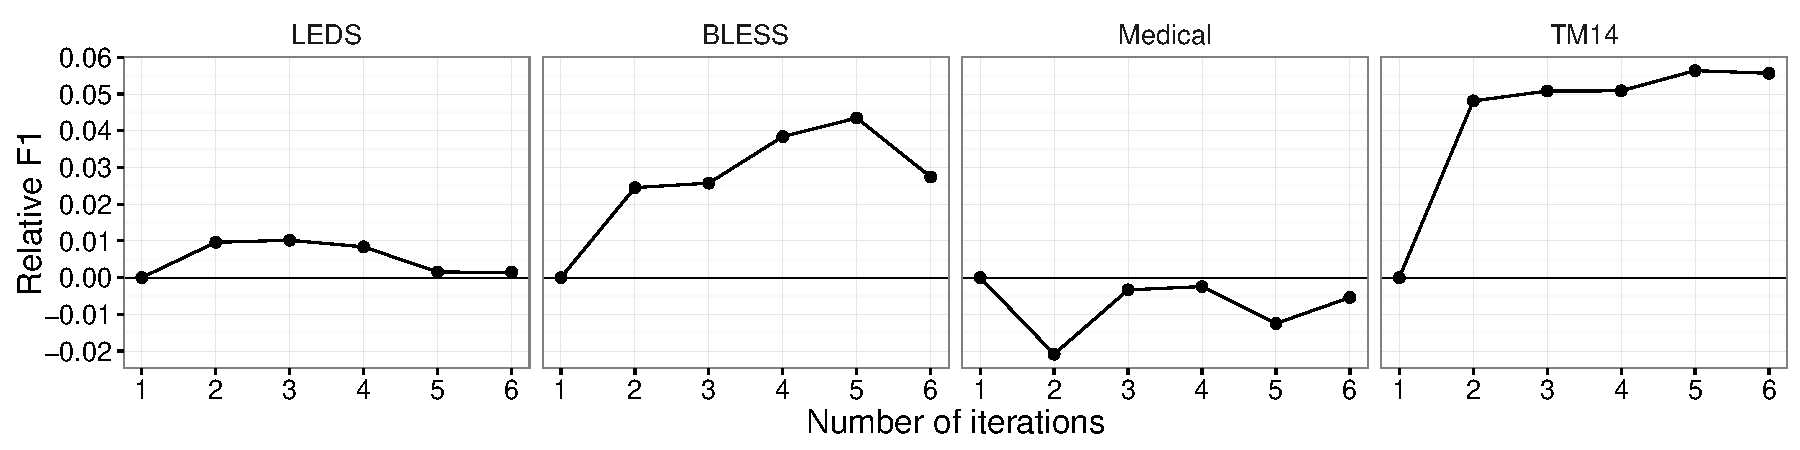
\includegraphics[width=1.00\textwidth]{plots/hpmbyiter}
\end{center}
\caption{Performance of model on development folds by number of iterations. Plots
show the improvement (absolute difference) in mean F1 over the model fixed at one
iteration.}
\label{fig:byiteration}
\end{figure*}

\begin{table*}
  \begin{center}
  \begin{small}
  \begin{tabular}{|ll|}
    \hline
    {\bf Iteration 1} & {\bf Iteration 2}\\
    \hline
    \ctx{nmod:such\_as+submarine}       &\ctx{nmod:including+animal}         \\
    \ctx{nmod:such\_as+ship}            &\ctx{nmod:including+snail}          \\
    \ctx{nmod:such\_as+seal}            &\ctx{nmod:including+insect}         \\
    \ctx{nmod:such\_as+plane}           &\ctx{nmod:such\_as+crustacean}      \\
    \ctx{nmod:such\_as+rack}            &\ctx{nmod:such\_as+mollusc}         \\
    \ctx{nmod:such\_as+rope}            &\ctx{nmod:such\_as+insect}          \\
   %\ctx{nmod:such\_as+box}             &\ctx{nmod:such\_as+animal}          \\
   %\ctx{nmod:such\_as+bat}             &\ctx{nmod:including+crustacean}     \\
   %\ctx{nmod:such\_as+pot}             &\ctx{nmod:including+amphibian}      \\
   %\ctx{nmod:such\_as+container}       &\ctx{nmod:including+pet}            \\
    \hline
    \hline
    {\bf Iteration 3} & {\bf Iteration 4}\\
    \hline
    \ctx{amod+free-swimming}            &\ctx{advcl+crown}                        \\
    \ctx{nmod:including\depinv+thing}   &\ctx{advcl+victorious}                   \\
    \ctx{nsubj\depinv+scarcer}          &\ctx{nsubj+eaters}                       \\
    \ctx{nsubj\depinv+pupate}           &\ctx{nsubj+kaine}                        \\
    \ctx{nmod:such\_as+mollusc}         &\ctx{nmod:at+finale}                     \\
    \ctx{nmod:of\depinv+value}          &\ctx{nsubj+gowen}                        \\
   %\ctx{nmod:as\depinv+exhibit}        &\ctx{nsubj+pillman}                      \\
   %\ctx{nmod:as\depinv+organism}       &\ctx{nmod:including\depinv+origin}       \\
   %\ctx{nmod:of\depinv+fecundity}      &\ctx{nmod:in+aa}                         \\
   %\ctx{nmod:as\depinv+feed}           &\ctx{nmod:of\depinv+stock}               \\
    \hline
  \end{tabular}
  \end{small}
\end{center}
\caption{Most similar contexts to the H-feature detector for each iteration
of the PCA-like procedure. This model was trained on all data of BLESS. The first and second
iterations contain clear Hearst patterns, while the third and fourth contain
some data-specific and non-obvious signals.}
\label{tab:multiter}
\end{table*}

In order to evaluate how the iterative feature extraction affects model
performance, we fix the regularization parameter at $C = 1$, and train our
model fixing the number of iterations to $n = \{1, \ldots, 6\}$.
We then measure the mean F1 score across the development folds and compare to a
baseline which uses only one iteration. Figure~\ref{fig:byiteration} shows
these results across all four datasets, with the 0 line set at performance of
the $n = 1$ baseline. Models above 0 benefit from the additional
iterations, while models below do not.

In the figure, we see that the iterative procedure moderately improves
performance LEDS, while greatly improving the scores of BLESS and TM14, but
on the medical dataset, additional iterations actually hurt performance.
The differing curves indicate that the optimal number of iterations is very
dataset specific, and provides differing amounts of improvement, and therefore
should be tuned carefully. The LEDS and BLESS curves indicate a sort of
``sweet spot'' behavior, where further iterations degrade performance.

To gain some additional insight into what is captured by the various iterations
of the feature extraction procedure, we repeat the procedure from
Section~\ref{sec:motivation}: we train our model on the entire BLESS dataset
using a fixed four iterations and regularization parameter. For each iteration,
we compare its learned H-feature detector to the context embeddings, and report
the most similar contexts for each iteration in Table~\ref{tab:multiter}.

The first iteration is identical to the one in Table~\ref{tab:ctxsim}, as
expected. The second iteration includes many H-features not picked up by the
first iteration, mostly those of the form \lit{[animals] including [cats]}. The
third iteration picks up some dataset specific signal, like \lit{free-swimming
[animal]} and \lit{value of [computer]}, and so on. By the fourth iteration,
the features no longer exhibit any obvious Hearst patterns, perhaps exceeding
the sweet spot we observed in Figure~\ref{fig:byiteration}.  Nonetheless, we
see how multiple iterations of the procedure allows our model to capture many
more useful features than a single Concat classifier on its own.

\section{Comparing to Path-based Entailment Detectors}

We have thus far shown that our proposed model strongly outperforms other
models for detecting hypernymy relations and lexical entailments using
distributional semantics. However, as discussed in earlier chapters, there
exists a wide literature in detecting lexical entailments directly using
Hearst patterns \cite{hearst:1992:coling} or their Dependency path
equivalents \cite{snow:2004:nips,girju:2006:cl}. These Hearst approaches are
known to produce low recall, since words do not always appear with their
hypernyms; yet Hearst approaches also may be complimented by distributional
approaches.
One recent line of work called HypeNET \cite{shwartz:2016:acl} aims to obtain
the best of both worlds, by integrating both path-based and distributional
based methods together using modern neural network techniques.

For a given pair of words $(h, w)$, HypeNET extracts the complete set of
dependency paths connecting $h$ and $w$ in any sentence in a large corpus.
These paths are then encoded into vectors using Long Short Term Memory networks
\cite{hochreiter:1997:nc}, and averaged together to obtain a final vector
representing the potential Hearst patterns between $h$ and $w$.  This path
vector is learned to maximize performance a set of binary
hypernymy/non-hypernymy training pairs. The Path vector may be evaluated
directly (``Path-based only''), or concatenated with distributional
representations of $h$ and $w$ (``Hybrid Path and Dist.'').
\newcite{shwartz:2016:acl} find a Hybrid approach outperforms Path-only and
Distributional-only comparisons.

We aim to directly compare with this approach by evaluating our model using
the same data and experimental setup used by \newcite{shwartz:2016:acl}.
They use a custom dataset of hypernymy pairs extracted from a union of several
datasets (including BLESS and DBPedia), and use only {\em related} words
as negative examples, preventing simple cosine baselines from doing well.
The full dataset contains about 70k pairs, roughly 25\% of which are positively
entailing.

\newcite{shwartz:2016:acl} evaluate in both a random-split and
zero lexical overlap settings, arguing that both are important: random-split
measures our ability to {\em complete} an existing taxonomy, while
zero lexical overlap measures ability to {\em induce} a taxonomy.
They use fixed 70\% train, 5\% validation, and 25\% test folds, which they
publish along with their paper.  Table~\ref{tab:shwartz}(a) shows the reported
results for a linear distributional-only baseline (Concat), along with their
novel Path-only model and state-of-the-art Hybrid model.

To compare our H-feature model to theirs, we use their published datasets,
and evaluate using the same training/test splits, and select hyperparameters
using the same validation sets. Since not all words in the dataset appear
in our set of distributional vectors, we assign out-of-vocabulary words
the ${\bf 0}$ vector. We evaluate using Concat, so the only difference between
our baseline and theirs is the choice of distributional vectors. We also
evaluate our H-feature model. 

\begin{table}
  \centering
  \begin{tabular}{|l|ccc|ccc|}
  \hline
  & \multicolumn{3}{ c|}{\bf Random Split} & \multicolumn{3}{c|}{\bf No Overlap}\\
  & {\bf P} & {\bf R} & {\bf F1} & {\bf P} & {\bf R} & {\bf F1}\\
  \hline
  Concat                    &    .901 &    .637 &    .746 &    .754 &    .551 &    .637 \\
  Path-based only           &    .811 &    .716 &    .761 &    .691 &    .632 &    .660 \\
  Hybrid Path and Dist.     &    .913 &{\bf.890}&{\bf.901}&{\bf.809}&    .617 &    .700 \\
  \hline
  \multicolumn{7}{c}{}\\
  [-0.5em]
  \multicolumn{7}{c}{(a) Reported results from \newcite{shwartz:2016:acl}.}\\
  \multicolumn{7}{c}{}\\
  \hline
  & \multicolumn{3}{ c|}{\bf Random Split} & \multicolumn{3}{c|}{\bf No Overlap}\\
  & {\bf P} & {\bf R} & {\bf F1} & {\bf P} & {\bf R} & {\bf F1}\\
  \hline
  Concat                    &    .910 &    .874 &    .892 &    .746 &    .949 &{\bf.836}\\
  H-feature model           &{\bf.926}&    .850 &    .886 &    .700 &{\bf.964}&    .811 \\
  \hline
  \multicolumn{7}{c}{}\\
  [-0.5em]
  \multicolumn{7}{c}{(b) Our results}\\
  \end{tabular}
  \caption{Comparing the H-feature model with Shwartz et al. (2016), a
    state-of-the-art system which combines a path-based with a distributional
  approach.}
  \label{tab:shwartz}
\end{table}

Table~\ref{tab:shwartz}(a) shows the reported results from
\newcite{shwartz:2016:acl}, and Table~\ref{tab:shwartz}(b) shows our results.
We see that our Concat and H-feature models both have a substantially higher F1
score than any of the models tested by \newcite{shwartz:2016:acl} in the zero
lexical overlap setting, giving a new State-of-the-Art on this dataset. Since
our Concat model does substantially better than any of their models, our
improvements are likely due to the choice of distributional space.
\newcite{shwartz:2016:acl} chose to use pretrained GloVe embeddings
\cite{pennington:2014:emnlp}, which use a fixed bag-of-words context window of
10.  As we saw in Figure~\ref{fig:window}, a choice of syntactic distributional
vectors substantially outperforms a bag-of-words distributional space.
Interestingly, the Hybrid and Path-only models should encode the syntactic
paths entirely, but these results suggest that, when training in zero lexical
overlap settings, collapsed dependency embeddings already capture sufficient
statistics. 

We also see that the Hybrid model of \newcite{shwartz:2016:acl} moderately
outperforms both of our models in the Random split setting. This indicates that
the Hybrid approach is still better for taxonomy completion settings.

We also notice that our Concat model slightly outperforms the H-feature model
in both random and zero overlap settings. We found the H-feature model chose to
use only one iteration of feature extraction in hyperparameter validation,
possibly explaining why the Concat model slightly outperforms the H-feature
model. We manually inspected the H-features learned across several iterations
and found only the first iteration contained interesting Hearst pattern type
features (e.g., \ctx{such\_as}). We suspect that this may be an artifact of the
dataset's construction, which included noisy examples from several data
sources, but no random negative pairs.

\section{Detecting Multiple Relations}

In the previous sections, we focused on how H-features may be used to detect
lexical entailments, and models were trained with a binary positive and
negative system. Yet it is unclear whether H-features will also be useful
for performing multi-relation classification, where labels may consist of
several relations. On one hand, the task may appear to be harder, and Hearst
patterns for non-hypernymy relations are much more difficult \cite{girju:2006:cl}.
On the other hand, the negative examples in the above sections constituted
many kinds of relationships (random, co-hyponymy, meronomy) and distingiushing
between these may overall improve performance. Furthermore, the relations
discussed in the previous sections were {\em only} noun-noun relations; however,
a variety of {\em other} interesting relations exist, like
{\em object-attribute} (noun-adjective), or {\em event-object} (verb-noun).

We now consider the necessary modifications to extend our H-feature to
multi-relation settings, or apply it to relationships which contain more
diverse settings.

\subsection{Adapting H-models for Multi-relation settings}

In Section~\ref{sec:hfeatproposed}, we proposed iteratively training multiple
H-feature extractors through the use of vector rejection. During each iteration
of feature, we trained the linear hyperplane $\vhatp = \wordpair$ which maximized
predictive accuracy. Since we trained a binary classifier and we wished to
positively identify hypernyms, we always selected the $\vhath$ vector at
each iteration, as it was the only logical hyperplane to choose.

With multi-class settings, the choice of which hyperplane is muddied: for
some relations, the choice between $\vhath$ and $\vhatw$ may not be as obvious:
perhaps some H-features are better learned from the RHS. Additionally,
since we are performing multi-class prediction, any linear model will
necessarily produce many different hyperplanes. In the one-versus-rest
training setting we opt for, we will learn $n$ hyperplanes for each of the
$n$ possible relation labels. With these two choices combined, each iteration
will have $2n$ possible H-feature choices.

We considered several options for how to select among the hyperplanes available
for H-features, and selected a simple heuristic which appeared to consistently
deliver quality H-features for several iterations: at each iteration, we select
the hyperplane with the largest vector magnitude. Intuitively, this heuristic
selects the most {\em pronounced} H-feature detector at each setting, and
we find this heuristic works well in practice.

Covering multiple relations additionally requires that we handle some
non-noun lexical items. Since datasets are not explicitly annotated with
part-of-speech tags, but our word vectors are, it is not obvious when we
see a word like \lit{show} whether we should select \lit{show/NN} or
\lit{show/VB}. We address this by always selecting the vector corresponding
to a word's {\em most common} POS tag. For example, since \lit{show/VB} is
more common in our corpus than \lit{show/NN}, we always select \lit{show/VB}
as our representation for \lit{show}.

\subsection{Data and Experiments}

We evaluate our multi-relation H-feature detector on several existing datasets covering a wide variety of relations.

The first dataset we use is {\bf BLESS} \cite{baroni:2011:gems}, which was also used
in the single-class experiments; previously, we only used the Hypernymy labels
as positive classes, and all other labels as negative. Here, we include all
relations with their positive labels, including the {\em attribute} and
{\em event} relations which were excluded in previous settings.

The second dataset we use is {\bf EVAL} \cite{santus:2015:ws}, which contains
a wide variety of lexical relations: {\em hypernymy}, {\em antonymy}, {\em
synonymy}, {\em has} (\lit{map} has \lit{information}), {\em property}
(\lit{volcano} has the property \lit{hot}), and {\em material} (\lit{clothes}
are {made of} \lit{cotton}).  The full dataset has 7,378 annotated pairs.
Notably, EVAL lacks any random negative pairs, meaning that all pairs contain
words semantically related in some way.

The third dataset we use is {\bf Root9} \cite{santus:2016:lrec} contains
12,763 pairs consisting of {\em random}, {\em hypernymy}, and {\em co-hyponymy}
relations. The dataset was intentionally constructed to be balance random
relations with non-random relations, and balance the non-random relations
equally between hypernymy and co-hyponymy.

The final dataset we use is {\bf K\&H+N} \cite{necsulescu:2015:starsem}, our
largest dataset containing of 57,510 annotated pairs consisting of {\em
hypernymy}, {\em co-hyponymy}, {\em meronomy}, and {\em random} relations and
covering three domains (animals, plants, and vehicles). Similar to BLESS and
LEDS, this dataset was extracted from WordNet, and was constructed to emphasize
identifying relations between words which {\em do not co-occur} in the BNC. The
K\&H+N name derives from the dataset introduced by \cite{kozareva:2010:emnlp},
and extended by \newcite{necsulescu:2015:starsem} to include the co-hyponymy
and meronomy.  The resulting dataset is extremely unbalanced, but still
contains over 1,000 meronomy examples and 4,000 hypernymy examples.

The distribution of each of the relations of each of the four datasets may
be found in Table~\ref{tab:multimakeup}.

\begin{table}
\centering
\begin{footnotesize}
\begin{tabular}{|lr|lr|lr|lr|}
  \hline
  \multicolumn{2}{|c|}{{\bf EVAL}} & \multicolumn{2}{c|}{{\bf BLESS}} & \multicolumn{2}{c|}{{\bf Root9}} & \multicolumn{2}{c|}{{\bf K\&H}}\\
  \hline
  \hline
  Hypernymy & 25.5\% & Hypernymy   &  5.0\% & Hypernymy   & 25.0\% & Hypernymy   &  7.5\% \\
  Antonym   & 21.7\% & Co-hyp      & 13.4\% & Co-hyp      & 25.1\% & Co-hyp      & 44.9\% \\
  Synonym   & 14.7\% & Meronomy    & 11.1\% & Random      & 49.9\% & Meronomy    &  1.8\% \\
  Has A     &  7.4\% & Attribute   & 10.3\% &             &        & Random      & 45.9\% \\
  Material  &  4.3\% & Event       & 14.4\% &             &        &             &        \\
  Property  & 17.6\% & Random      & 45.8\% &             &        &             &        \\
  Part Of   &  8.9\% &             &        &             &        &             &        \\
  \hline
\end{tabular}
\end{footnotesize}
\caption{The makeup of each of the four multi-relation datasets, by relation type. Not}
\label{tab:multimakeup}
\end{table}

\subsection{Experiments}

We follow the same experimental setup described in Section~\ref{sec:singleexp}.
Datasets are divided into a 20-fold Cross Validation setting with zero lexical
overlap, with rotating validation and testing folds. We report mean {\em
accuracy} across all folds, as F1 is poorly suited for non-binary datasets.
We use balanced class weights for both H-feature extraction, and training
the final meta-classifier, and tune the regularization parameter in
$C = \{10^{-4}, \ldots, 10^{4}\}$ and number of iterations $N = \{1, \ldots,
10\}$ using grid search. We found it necessary to increase the maximum number
of iterations to 10 (from 6 in the binary experiments), as the larger datasets
and more diverse relations required additional H-features.

We compare our model with the same baselines and prior work as done in our own
binary experiments. We note that many of these baselines have never been
applied to these datasets before.

\begin{table}
\centering
\begin{tabular}{|l|rrrr|}
  \hline
  {\bf Model}      & {\bf EVAL}  & {\bf BLESS} & {\bf Root9} & {\bf K\&H}  \\
  \hline
  \hline
  \multicolumn{5}{|c|}{Linear Models}\\
  \hline
  Concat           &      .469   &      .665   &      .581     &      .716   \\
  Diff             &      .442   &      .600   &      .514     &      .697   \\
  Asym             &      .453   &      .602   &      .671     &      .718   \\
  Concat+Diff      &      .459   &      .690   &      .596     &      .708   \\
  Concat+Asym      &      .464   &      .688   &      .644     &      .709   \\
  \hline
  \multicolumn{5}{|c|}{Nonlinear Models}\\
  \hline
  RBF              &      .455   &      .625   &      .560     &      .739   \\
  Ksim             &      .459   &      .633   &      .657     &      .744   \\
  H-feature Model  &  {\bf.470}  &  {\bf.713}  &  {\bf.732}    &  {\bf.755}  \\
  \hline
\end{tabular}
\caption{Mean Accuracy scores for each model and dataset for multi-relation classification.}
\label{tab:multiresults}
\end{table}

Table~\ref{tab:multiresults} shows the results of our experiments in
multi-relation classification. We see that our H-feature model has the
strongest performance in all four datasets. Our model only slightly
(non-significantly) improves over the Concat baseline in the EVAL dataset.
In the remaining three datasets, our H-feature model improves over the
next-strongest model by a significant margin (McNemar test, $p < .01$).
Clearly, the H-feature model is more adept at identifying lexical relations
than our baselines.

We may also analyze the H-features extracted by each of the iterations of the
model. We train an H-feature model on each of the four datasets with 10
iterations of H-feature extraction. We compared each of these 40 H-features
with their most similar contexts, and manually filtered the list to the
8 most interesting H-feature sets. We observed several hypernymy H-feature
sets similar to those in Table~\ref{tab:ctxsim}, and excluded those from our
consideration.
Table~\ref{tab:ctxsimmulti} lists our 8 H-features, along with the dataset
each was extracted from, which iteration it was learned in, and which relation
it provides evidence for. In general, we found the H-features of the BLESS
dataset to be higher quality and more interesting than other datasets, but
we report at least one H-feature from each.

\begin{table}[t]
\centering
\begin{small}
\begin{tabular}{|ll|}
\hline
{\bf BLESS: Co-hyponymy (Itr. 2)}     & {\bf BLESS: Meronomy (Itr. 3)}        \\
\hline
\ctx{nmod:between\depinv+cross}       & \ctx{amod+splayed}                    \\
\ctx{nmod:like\depinv+vaguely}        & \ctx{amod+swept-back}                 \\
\ctx{amod+trusty}                     & \ctx{amod+low-set}                    \\
\ctx{nmod:between\depinv+hybrid}      & \ctx{dobj\depinv+protrude}            \\
\ctx{compound+striped}                & \ctx{amod+upswept}                    \\
\ctx{nmod:like\depinv+pull}           & \ctx{nmod:with\depinv+distinctive}    \\
%\ctx{nmod:like\depinv+design}         & \ctx{appos+underside}                 \\
%\ctx{amod+talk}                       & \ctx{nmod:by+alcalde}                 \\
%\ctx{nmod:like\depinv+carry}          & \ctx{nmod:to\depinv+tinge}            \\
%\ctx{acl+outfit}                      & \ctx{nmod:with\depinv+fuselage}       \\
\hline
\hline
{\bf BLESS: Attribute (Itr. 4)}       & {\bf BLESS: Event (Itr. 6)}           \\
\hline
\ctx{amod\depinv+broom}               & \ctx{nmod:to\depinv+chance}           \\
\ctx{amod\depinv+cutlass}             & \ctx{acl:relcl\depinv+fowl}           \\
\ctx{amod\depinv+pail}                & \ctx{nsubj+weta}                      \\
\ctx{amod\depinv+muff}                & \ctx{acl:relcl\depinv+hen}            \\
\ctx{amod\depinv+paintbrush}          & \ctx{nmod:to\depinv+enough}           \\
\ctx{amod\depinv+aga}                 & \ctx{nmod:to\depinv+reason}           \\
%\ctx{amod\depinv+woody}               & \ctx{nmod:to\depinv+daring}           \\
%\ctx{amod\depinv+bodied}              & \ctx{nmod:to\depinv+afraid}           \\
%\ctx{advmod+unnaturally}              & \ctx{nmod:between+dusk}               \\
%\ctx{amod\depinv+kettle}              & \ctx{acl\depinv+ready}                \\
\hline
\hline
{\bf EVAL: Material (Itr. 2)}         & {\bf EVAL: Has A (Itr. 3)}         \\
\hline
\ctx{nmod:from\depinv+handcraft}      & \ctx{nmod:with\depinv+one}            \\
\ctx{nmod:of\depinv+fashion}          & \ctx{nmod:below\depinv+have}          \\
\ctx{nmod:out\_of\depinv+construct}   & \ctx{nmod:above\depinv+have}          \\
\ctx{nmod:like\depinv+material}       & \ctx{nmod:with\depinv+long}           \\
\ctx{nmod:out\_of\depinv+fashion}     & \ctx{nmod:with\depinv+long}           \\
\ctx{appos+fiber}                     & \ctx{nmod:with\depinv+larger}         \\
%\ctx{nmod:than\depinv+material}       & \ctx{nmod:with\depinv+type}           \\
%\ctx{nmod:npmod\depinv+clad}          & \ctx{nmod:below\depinv+make}          \\
%\ctx{nmod:such\_as\depinv+fibre}      & \ctx{nmod:with\depinv+body}           \\
%\ctx{compound\depinv+fiber}           & \ctx{compound\depinv+downward}        \\
\hline
\hline
{\bf K\&H: Meronomy (Itr. 3)}         & {\bf Root9: Co-hyponymy (Itr. 1)}     \\
\hline
\ctx{nmod:poss+stallion}              & \ctx{nmod:as\depinv+big}              \\
\ctx{nmod:poss+serpent}               & \ctx{nmod:between\depinv+cross}       \\
\ctx{nmod:with-1+beast}               & \ctx{nmod:such\_as\depinv+variety}    \\
\ctx{nmod:poss+lion}                  & \ctx{nmod:like\depinv+pull}           \\
\ctx{nmod:poss+hog}                   & \ctx{amod+trusty}                     \\
\ctx{nmod:poss+lizard}                & \ctx{nmod:between\depinv+hybrid}      \\
%\ctx{nmod:with-1+bull}                & \ctx{amod+proverbial}                 \\
%\ctx{nmod:of+stag}                    & \ctx{compound+striped}                \\
%\ctx{nmod:of+leviathan}               & \ctx{nmod:like\depinv+one}            \\
%\ctx{nmod:poss+shark}                 & \ctx{xcomp\depinv+resemble}           \\
\hline
\end{tabular}
\end{small}
\caption{Feature detectors for different relations learned by our model in a
  variety of datasets. These 8 hyperplanes were selected as most interesting
  among 40. Each hyperplane is listed with its corresponding dataset,
  identifying relation, and which iteration it was extracted from. Several
  Hypernymy hyperplanes were also observed, but are not shown here.}
\label{tab:ctxsimmulti}
\end{table}

In general, we find the H-features in the multi-relation settings are strong
identifiers of their corresponding relations. Many are not as obvious or as
clear cut as the original Hypernymy H-features, but all are interesting
nonetheless. The BLESS and Root9 co-hyponymy detectors identify some
interesting patterns from genetics, like \lit{cross between [tomato] and
[tobacco]} and \lit{[cat] vaguely like a [dog]}. The K\&H meronomy H-features
identifies clear possessive constructions (\lit{stallion's [tail]}) and mirror
the meronomy patterns proposed by \newcite{girju:2006:cl}, though
the contexts are strongly biased towards by its animal-heavy construction.
The EVAL Material detector identifies strong material patterns
(\lit{[bookshelves] handcrafted from [wood]}), and the EVAL Has detector
identifies simple prepositional phrases (\lit{[garden] with one [flower]}).
Altogether, we see some strong evidence that the H-features truly are
indicative of the relations they are meant to identify, indicating our
proposed model works strongly in multi-relation settings.

Some of the H-features are more prototypical than the others, and their
most similar words (rather than contexts) tend to appear directly in the data.
For example, the BLESS Meronomy H-feature identifies many features that are
common of animal parts, like \lit{splayed [feet]} or \lit{swept back [wings]}.
The BLESS Attribute H-feature learned to identify color words, so its contexts
are mostly concrete nouns which are described using these colors. The BLESS
Event hyperplane appears only to segment verbs from the rest of the data,
with contexts like \lit{chance to [eat]} or \lit{enough to [eat]}. This is
unsurprising, as this was the only relation with any examples of verbs.
Although these contexts tend toward prototypicality, it is also clear why
they should be useful for the various relationships.

\section{Chapter Summary}

In this chapter, we proposed a new model for detecting lexical relationships
using distributional vectors. We showed that the choice of bag-of-words
or syntactic embeddings has a large impact on performance of a baseline
Concat model. We then showed that the Concat model may be interpreted by
comparing its hyperplane in the embedded {\em context} space. We found
this interpretation gives direct evidence as an Hearst-like feature extractor,
explaining Concat's high performance.

We propose our H-feature
model, which exploits this behavior through repeated iterations of feature
extraction in a PCA-like procedure, and learns a final classifier which obtains
state-of-the-art performance on several datasets. We also compare our model
to a state-of-the-art Hybrid path-and-distributional model, and found our
model substantially outperforms the Hybrid model in an experimental setting
with zero lexical overlap. Finally, we show the necessary extensions to our
model in order to use it for multi-relation classification settings. We found
our model outperforms baselines and the prior work on four datasets, and that
the model learns interesting H-features corresponding to a variety of
lexical relations.

